%  LaTeX support: latex@mdpi.com 
%  For support, please attach all files needed for compiling as well as the log file, and specify your operating system, LaTeX version, and LaTeX editor.
%=================================================================

\documentclass[
  futuretransp,
  submit,
  moreauthors,
]{Definitions/mdpi}
%--------------------
% Class Options:
%--------------------
%----------
% journal
%----------
% Choose between the following MDPI journals:
% acoustics, actuators, addictions, admsci, adolescents, aerobiology, aerospace, agriculture, agriengineering, agrochemicals, agronomy, ai, air, algorithms, allergies, alloys, analytica, analytics, anatomia, animals, antibiotics, antibodies, antioxidants, applbiosci, appliedchem, appliedmath, applmech, applmicrobiol, applnano, applsci, aquacj, architecture, arm, arthropoda, arts, asc, asi, astronomy, atmosphere, atoms, audiolres, automation, axioms, bacteria, batteries, bdcc, behavsci, beverages, biochem, bioengineering, biologics, biology, biomass, biomechanics, biomed, biomedicines, biomedinformatics, biomimetics, biomolecules, biophysica, biosensors, biotech, birds, bloods, blsf, brainsci, breath, buildings, businesses, cancers, carbon, cardiogenetics, catalysts, cells, ceramics, challenges, chemengineering, chemistry, chemosensors, chemproc, children, chips, cimb, civileng, cleantechnol, climate, clinpract, clockssleep, cmd, coasts, coatings, colloids, colorants, commodities, compounds, computation, computers, condensedmatter, conservation, constrmater, cosmetics, covid, crops, cryptography, crystals, csmf, ctn, curroncol, cyber, dairy, data, ddc, dentistry, dermato, dermatopathology, designs, devices, diabetology, diagnostics, dietetics, digital, disabilities, diseases, diversity, dna, drones, dynamics, earth, ebj, ecologies, econometrics, economies, education, ejihpe, electricity, electrochem, electronicmat, electronics, encyclopedia, endocrines, energies, eng, engproc, entomology, entropy, environments, environsciproc, epidemiologia, epigenomes, est, fermentation, fibers, fintech, fire, fishes, fluids, foods, forecasting, forensicsci, forests, foundations, fractalfract, fuels, future, futureinternet, futurepharmacol, futurephys, futuretransp, galaxies, games, gases, gastroent, gastrointestdisord, gels, genealogy, genes, geographies, geohazards, geomatics, geosciences, geotechnics, geriatrics, grasses, gucdd, hazardousmatters, healthcare, hearts, hemato, hematolrep, heritage, higheredu, highthroughput, histories, horticulturae, hospitals, humanities, humans, hydrobiology, hydrogen, hydrology, hygiene, idr, ijerph, ijfs, ijgi, ijms, ijns, ijpb, ijtm, ijtpp, ime, immuno, informatics, information, infrastructures, inorganics, insects, instruments, inventions, iot, j, jal, jcdd, jcm, jcp, jcs, jcto, jdb, jeta, jfb, jfmk, jimaging, jintelligence, jlpea, jmmp, jmp, jmse, jne, jnt, jof, joitmc, jor, journalmedia, jox, jpm, jrfm, jsan, jtaer, jvd, jzbg, kidneydial, kinasesphosphatases, knowledge, land, languages, laws, life, liquids, literature, livers, logics, logistics, lubricants, lymphatics, machines, macromol, magnetism, magnetochemistry, make, marinedrugs, materials, materproc, mathematics, mca, measurements, medicina, medicines, medsci, membranes, merits, metabolites, metals, meteorology, methane, metrology, micro, microarrays, microbiolres, micromachines, microorganisms, microplastics, minerals, mining, modelling, molbank, molecules, mps, msf, mti, muscles, nanoenergyadv, nanomanufacturing,\gdef\@continuouspages{yes}} nanomaterials, ncrna, ndt, network, neuroglia, neurolint, neurosci, nitrogen, notspecified, %%nri, nursrep, nutraceuticals, nutrients, obesities, oceans, ohbm, onco, %oncopathology, optics, oral, organics, organoids, osteology, oxygen, parasites, parasitologia, particles, pathogens, pathophysiology, pediatrrep, pharmaceuticals, pharmaceutics, pharmacoepidemiology,\gdef\@ISSN{2813-0618}\gdef\@continuous pharmacy, philosophies, photochem, photonics, phycology, physchem, physics, physiologia, plants, plasma, platforms, pollutants, polymers, polysaccharides, poultry, powders, preprints, proceedings, processes, prosthesis, proteomes, psf, psych, psychiatryint, psychoactives, publications, quantumrep, quaternary, qubs, radiation, reactions, receptors, recycling, regeneration, religions, remotesensing, reports, reprodmed, resources, rheumato, risks, robotics, ruminants, safety, sci, scipharm, sclerosis, seeds, sensors, separations, sexes, signals, sinusitis, skins, smartcities, sna, societies, socsci, software, soilsystems, solar, solids, spectroscj, sports, standards, stats, std, stresses, surfaces, surgeries, suschem, sustainability, symmetry, synbio, systems, targets, taxonomy, technologies, telecom, test, textiles, thalassrep, thermo, tomography, tourismhosp, toxics, toxins, transplantology, transportation, traumacare, traumas, tropicalmed, universe, urbansci, uro, vaccines, vehicles, venereology, vetsci, vibration, virtualworlds, viruses, vision, waste, water, wem, wevj, wind, women, world, youth, zoonoticdis 
% For posting an early version of this manuscript as a preprint, you may use "preprints" as the journal. Changing "submit" to "accept" before posting will remove line numbers.

%---------
% article
%---------
% The default type of manuscript is "article", but can be replaced by: 
% abstract, addendum, article, book, bookreview, briefreport, casereport, comment, commentary, communication, conferenceproceedings, correction, conferencereport, entry, expressionofconcern, extendedabstract, datadescriptor, editorial, essay, erratum, hypothesis, interestingimage, obituary, opinion, projectreport, reply, retraction, review, perspective, protocol, shortnote, studyprotocol, systematicreview, supfile, technicalnote, viewpoint, guidelines, registeredreport, tutorial
% supfile = supplementary materials

%----------
% submit
%----------
% The class option "submit" will be changed to "accept" by the Editorial Office when the paper is accepted. This will only make changes to the frontpage (e.g., the logo of the journal will get visible), the headings, and the copyright information. Also, line numbering will be removed. Journal info and pagination for accepted papers will also be assigned by the Editorial Office.

%------------------
% moreauthors
%------------------
% If there is only one author the class option oneauthor should be used. Otherwise use the class option moreauthors.

%---------
% pdftex
%---------
% The option pdftex is for use with pdfLaTeX. Remove "pdftex" for (1) compiling with LaTeX & dvi2pdf (if eps figures are used) or for (2) compiling with XeLaTeX.

%=================================================================
% MDPI internal commands - do not modify
\firstpage{1} 
\makeatletter 
\setcounter{page}{\@firstpage} 
\makeatother
\pubvolume{1}
\issuenum{1}
\articlenumber{0}
\pubyear{2024}
\copyrightyear{2024}
%\externaleditor{Academic Editor: Firstname Lastname}
\datereceived{ } 
\daterevised{ } % Comment out if no revised date
\dateaccepted{ } 
\datepublished{ } 
%\datecorrected{} % For corrected papers: "Corrected: XXX" date in the original paper.
%\dateretracted{} % For corrected papers: "Retracted: XXX" date in the original paper.
\hreflink{https://doi.org/} % If needed use \linebreak
%\doinum{}
%\pdfoutput=1 % Uncommented for upload to arXiv.org
%\CorrStatement{yes}  % For updates


%=================================================================
% Add packages and commands here. The following packages are loaded in our class file: fontenc, inputenc, calc, indentfirst, fancyhdr, graphicx, epstopdf, lastpage, ifthen, float, amsmath, amssymb, lineno, setspace, enumitem, mathpazo, booktabs, titlesec, etoolbox, tabto, xcolor, colortbl, soul, multirow, microtype, tikz, totcount, changepage, attrib, upgreek, array, tabularx, pbox, ragged2e, tocloft, marginnote, marginfix, enotez, amsthm, natbib, hyperref, cleveref, scrextend, url, geometry, newfloat, caption, draftwatermark, seqsplit
% cleveref: load \crefname definitions after \begin{document}




\providecommand{\tightlist}{%
  \setlength{\itemsep}{0pt}\setlength{\parskip}{0pt}}
\usepackage{longtable,booktabs,array}
\usepackage{calc} % for calculating minipage widths
% Correct order of tables after \paragraph or \subparagraph
\usepackage{etoolbox}
\makeatletter
\patchcmd\longtable{\par}{\if@noskipsec\mbox{}\fi\par}{}{}
\makeatother
% Allow footnotes in longtable head/foot
\IfFileExists{footnotehyper.sty}{\usepackage{footnotehyper}}{\usepackage{footnote}}
\makesavenoteenv{longtable}

\usepackage{graphicx}
\makeatletter
\newsavebox\pandoc@box
\newcommand*\pandocbounded[1]{% scales image to fit in text height/width
  \sbox\pandoc@box{#1}%
  \Gscale@div\@tempa{\textheight}{\dimexpr\ht\pandoc@box+\dp\pandoc@box\relax}%
  \Gscale@div\@tempb{\linewidth}{\wd\pandoc@box}%
  \ifdim\@tempb\p@<\@tempa\p@\let\@tempa\@tempb\fi% select the smaller of both
  \ifdim\@tempa\p@<\p@\scalebox{\@tempa}{\usebox\pandoc@box}%
  \else\usebox{\pandoc@box}%
  \fi%
}
% Set default figure placement to htbp
\def\fps@figure{htbp}
\makeatother

% definitions for citeproc citations
\NewDocumentCommand\citeproctext{}{}
\NewDocumentCommand\citeproc{mm}{%
  \begingroup\def\citeproctext{#2}\cite{#1}\endgroup}
\makeatletter
 % allow citations to break across lines
 \let\@cite@ofmt\@firstofone
 % avoid brackets around text for \cite:
 \def\@biblabel#1{}
 \def\@cite#1#2{{#1\if@tempswa , #2\fi}}
\makeatother
\newlength{\cslhangindent}
\setlength{\cslhangindent}{1.5em}
\newlength{\csllabelwidth}
\setlength{\csllabelwidth}{3em}
\newenvironment{CSLReferences}[2] % #1 hanging-indent, #2 entry-spacing
 {\begin{list}{}{%
  \setlength{\itemindent}{0pt}
  \setlength{\leftmargin}{0pt}
  \setlength{\parsep}{0pt}
  % turn on hanging indent if param 1 is 1
  \ifodd #1
   \setlength{\leftmargin}{\cslhangindent}
   \setlength{\itemindent}{-1\cslhangindent}
  \fi
  % set entry spacing
  \setlength{\itemsep}{#2\baselineskip}}}
 {\end{list}}
\usepackage{calc}
\newcommand{\CSLBlock}[1]{\hfill\break\parbox[t]{\linewidth}{\strut\ignorespaces#1\strut}}
\newcommand{\CSLLeftMargin}[1]{\parbox[t]{\csllabelwidth}{\strut#1\strut}}
\newcommand{\CSLRightInline}[1]{\parbox[t]{\linewidth - \csllabelwidth}{\strut#1\strut}}
\newcommand{\CSLIndent}[1]{\hspace{\cslhangindent}#1}


\usepackage{booktabs}
\usepackage{longtable}
\usepackage{array}
\usepackage{multirow}
\usepackage{wrapfig}
\usepackage{float}
\usepackage{colortbl}
\usepackage{pdflscape}
\usepackage{tabu}
\usepackage{threeparttable}
\usepackage{threeparttablex}
\usepackage[normalem]{ulem}
\usepackage{makecell}
\usepackage{xcolor}
\makeatletter
\@ifpackageloaded{bookmark}{}{\usepackage{bookmark}}
\makeatother
\makeatletter
\@ifpackageloaded{caption}{}{\usepackage{caption}}
\AtBeginDocument{%
\ifdefined\contentsname
  \renewcommand*\contentsname{Table of contents}
\else
  \newcommand\contentsname{Table of contents}
\fi
\ifdefined\listfigurename
  \renewcommand*\listfigurename{List of Figures}
\else
  \newcommand\listfigurename{List of Figures}
\fi
\ifdefined\listtablename
  \renewcommand*\listtablename{List of Tables}
\else
  \newcommand\listtablename{List of Tables}
\fi
\ifdefined\figurename
  \renewcommand*\figurename{Figure}
\else
  \newcommand\figurename{Figure}
\fi
\ifdefined\tablename
  \renewcommand*\tablename{Table}
\else
  \newcommand\tablename{Table}
\fi
}
\@ifpackageloaded{float}{}{\usepackage{float}}
\floatstyle{ruled}
\@ifundefined{c@chapter}{\newfloat{codelisting}{h}{lop}}{\newfloat{codelisting}{h}{lop}[chapter]}
\floatname{codelisting}{Listing}
\newcommand*\listoflistings{\listof{codelisting}{List of Listings}}
\makeatother
\makeatletter
\makeatother
\makeatletter
\@ifpackageloaded{caption}{}{\usepackage{caption}}
\@ifpackageloaded{subcaption}{}{\usepackage{subcaption}}
\makeatother
%=================================================================
% Please use the following mathematics environments: Theorem, Lemma, Corollary, Proposition, Characterization, Property, Problem, Example, ExamplesandDefinitions, Hypothesis, Remark, Definition, Notation, Assumption
%% For proofs, please use the proof environment (the amsthm package is loaded by the MDPI class).

%=================================================================


%=================================================================
% Full title of the paper (Capitalized)
\Title{Evaluating the Impacts of Parameter Uncertainty in a Practical
Transportation Demand Model}

% MDPI internal command: Title for citation in the left column
\TitleCitation{Evaluating the Impacts of Parameter Uncertainty in a
Practical Transportation Demand Model}

\abstract{The inherent uncertainty in travel forecasting models ---
arising from potential and unkown errors in input data, parameter
estimation, or model formulation --- is receiving increasing attention
from the scholarly and practicing community. In this research, we
investigate the variance in forecasted traffic volumes resulting from
varying the mode and destination choice parameters in an advanced
trip-based travel demand model. Using Latin hypercube sampling to
construct several hundred combinations of parameters across the
plausible parameter space, we introduce substantial changes to implied
travel impedances and modal utilities. However, the aggregate effects of
of these changes on forecasted traffic volumes is small, with a variance
of approximately 1 percent on high-volume facilities. It is likely that
in this example --- and perhaps in others --- the static network
assignment places constraints on the possible volume solutions and
limits the practical impacts of parameter uncertainty. Further research
should examine the robustness of this finding to other less constrained
networks and to activity-based travel model frameworks.}
\keyword{Travel modeling;
Uncertainty}


% this solution came from ihrke/mdpi
\newcommand{\orcidauthorB}{0000-0003-3999-7584} 

\Author{Natalie Gibbons$^{1}$~and~Gregory S. Macfarlane$^{2}$\orcidB{}
}

\AuthorNames{ Natalie Gibbons,  Gregory S. Macfarlane}

% address for the affiliations
\address {%
$^{1}$ \quad Kimley-Horn Associates\\
$^{2}$ \quad Civil and Construction Engineering, Brigham Young
University\\
}


\newcommand\getfirst[1]{\getfirstaux#1\relax} \def\getfirstaux#1#2\relax{#1}
\AuthorCitation{Gibbons, \getfirst{Natalie}.; Macfarlane, \getfirst{Gregory S.}.}
% Contact information of the corresponding author
\corres{Correspondence: gregmacfarlane@byu.edu}
%%%%%%%%%%%%%%%%%%%%%%%%%%%%%%%%%%%%%%%%%%
\begin{document}

\bookmarksetup{startatroot}

\section{Introduction}\label{introduction}

The inherent accuracy and uncertainty in travel forecasting models is
receiving increasing attention from the scholarly and practicing
community. Given that such models are used in the allocation of billions
of dollars of infrastructure financing each year, the financial risks
for inaccurate or imprecise forecasts are high (Flyvbjerg et al., 2005;
Voulgaris, 2019).

Transportation demand forecasting models, like other
mathematical-statistical models, might be abstracted to the following
basic form,

\[
y = f(X, \beta)
\]where \(y\) is the variable being predicted based on input data \(X\),
moderated through a specific functional form \(f()\) and parameters
\(\beta\). Three general sources of error may lead a forecast value
\(\hat{y}\) to differ from the ``true'' or ``actual'' value of \(y\)
(Rasouli and Timmermans, 2012):

\begin{enumerate}
\def\labelenumi{\arabic{enumi}.}
\tightlist
\item
  The input data \(X\) might contain errors, due to inaccuracies in the
  base year, or an inaccurate projection of land use, petroleum price,
  or other key input variable. This was among the primary issues
  identified by Hoque et al. (2021) in a historical analysis of the
  accuracy of travel forecasts.
\item
  The model form \(f()\) may be improperly specified. Variables that
  play a major role in travel behavior may not be included due to lack
  of information, or the unobserved error components may have a
  different correlation than was assumed during model development. A
  detailed description of specifying mode choice model variables and
  nesting of error structures is given by Koppelman and Bhat (2006).
\item
  The parameter estimates \(\hat{\beta}\) of the ``true'' parameters
  \(\beta\) may have incorrect values. This may be because the
  parameters were estimated on an improperly specified model \(f()\), or
  because the estimation dataset was improperly weighted.
\end{enumerate}

Of these potential sources of error, only the third is substantively
addressed in classical statistics. The standard errors of the model
parameter estimates in a theoretical perspective address the parameter
uncertainty question to a great degree. Yet even this source of
uncertainty has been largely ignored in transportation forecasts, and
model development documentation often elides the variance in these
values completely (National Academies of Sciences, Engineering, and
Medicine., 2012). Zhao and Kockelman (2002) examined the effects of this
parameter uncertainty in a trip-based model of a contrived 25 zone
region, but a systemic analysis of this uncertainty in a practical model
is not common.

In this research, we investigate the uncertainty in traffic forecasts
resulting from plausible parameter uncertainty in an advanced trip-based
transportation demand model. Using a Latin hypercube sampling (LHS)
methodology, we simulate one hundred potential parameter sets for a
combined mode and destination choice model in Roanoke, Virginia, USA. We
then assign the resulting trip matrices to the highway network for the
region and evaluate the PM and daily assigned traffic volumes alongside
the variation in implied impedance and accessibility.

This paper proceeds first with a description of the model design and
simulation sampling methodology in Chapter~\ref{sec-methods}, followed
by a discussion of the variation in mode, destination, and traffic
performance measures in Chapter~\ref{sec-results}. The paper concludes
in Chapter~\ref{sec-conclusions} with a summary of the key findings
alongside a presentation of limitations and related indications for
future research.

\bookmarksetup{startatroot}

\section{Literature Review}\label{literature-review}

Uncertainty has been examined in various ways over the last two decades,
and is becoming increasingly important for researchers. This review
looks at why uncertainty is important to evaluate in transportation
demand models, and research that has been done to evaluate uncertainty.
Rasouli and Timmermans (2012) has an extensive literature review on this
topic. An overview of the literature and which source of uncertainty
they evaluate can be found in Table~\ref{tbl-authors}.

\begin{longtable}[t]{ll}

\caption{\label{tbl-authors}Studies of Forecasting Uncertainty}

\tabularnewline

\toprule
Reference & Uncertainty Source(s) Evaluated\\
\midrule
@rodier2002uncertain & Input Data\\
@zhao2002 & Input Data \& Parameter Estimates\\
@clay2005univariate & Input Data \& Parameter Estimates\\
@flyvbjerg2005 & Model Form\\
@armoogum2009 & Model Form\\
\addlinespace
@duthie2010highway & Input Data \& Parameter Estimates\\
@welde2011planners & Model Form\\
@yang2013 & Input Data \& Parameter Estimates\\
@manzo2015 & Input Data \& Parameter Estimates\\
@petrik2016measuring & Input Data \& Parameter Estimates\\
\addlinespace
@petrik2020uncertainty & Model Form \& Parameter Estimates\\
@hoque2021 & Input Data\\
\bottomrule

\end{longtable}

Model accuracy is the basis for why uncertainty of input data and/or
parameter estimates are important to study. Travel forecasters have
always been cognizant of the uncertainty in their forecasts, especially
as project decisions are made using these models, often with high
financial impacts.

Flyvbjerg et al. (2005) collected data from various forecasting traffic
models with an emphasis on rail projects. They used the forecast data
for a given year and the actual value that was collected for the same
year. Their study found that there is a statistical significance in the
difference of the estimated and actual values. Rail projects are
generally overestimating passenger forecasts by 106\%, and half of road
projects have a traffic forecast difference of plus or minus 20\%. They
did not identify where this inaccuracy came from, but they identified
that it was important for future research.

Armoogum et al. (2009) looked at uncertainty within a forecasting model
for the Paris and Montreal metropolitan regions. The sources of
uncertainty analysed were calibration of the model, behavior of future
generations, and demographic projections. A jackknife technique, rather
than sampling methods, was used to estimated confidence intervals for
each source of error using multiple years of analysis. This technique is
a way to reduce the bias of an estimator and permits the estimation of
confidence intervals to produce variance estimates. They found that the
longer the forecasting period was, the larger the uncertainty. Generally
the model forecast within 10-15\%, reaching higher percentage ranges for
variables with small values or small sample sizes.

Welde and Odeck (2011) compared actual and forecast traffic values for
25 toll and 25 toll free roads in Norway. They evaluated the accuracy of
Norwegian transportation planning models over the years. Generally
traffic models overestimate traffic. This study found that toll
projects, on average, overestimated traffic, but only by an average of
2.5\%. Toll free projects, however, underestimated traffic by an average
of 19\%. They concluded that Norwegian toll projects have been fairly
accurate, with a probable cause coming from the scrutiny that planners
get when developing a toll project. A similar scrutiny should then also
be placed on toll free projects as they are significantly less accurate.

These articles show that models have errors which effects traffic
projections by a significant amount. These articles identified that
error existed but did not quantitatively identify the source of the
error. The most researched error source has been on model form but that
research has mostly been excluded in this review as it is not the main
focus of this research. The second most researched form has been on
input data. Chronologically, Rodier and Johnston (2002), Zhao and
Kockelman (2002), Clay and Johnston (2005), Duthie et al. (2010), Yang
et al. (2013), Manzo et al. (2015), and Petrik et al. (2016) have all
researched input error, with all but the first also looking at parameter
estimate error as well. Parameter estimation error has been the least
researched source of uncertainty, where there have been no studies
focused only on that source of error. Petrik et al. (2020) looked at
parameter estimates, but with a focus also on model form error. The
details of each study are described below in chronological order.

Rodier and Johnston (2002) looked at uncertainty in socioeconomic
projections (population and employment, household income, and petroleum
prices) at the county-level for the Sacramento, California region. They
wanted to know if the uncertainty in the range of plausible
socioeconomic values was a significant source of error in the projection
of future travel patterns and vehicle emissions. They identified ranges
for population and employment, household income, and petroleum price for
two scenario years (2005 and 2015). The ranges varied based on the
scenario year and the socioeconomic variable. They changed one variable
at a time for a total of 19 iterations of the model run for 2005 and 21
iterations for 2015. Their results indicated that the error in
projections for household income and petroleum prices is not a
significant source of uncertainty, but error ranges for population and
employment projections are a significant source for changes in travel
and emissions. The input data of population and employment were a
significant factor to the model result uncertainty.

Zhao and Kockelman (2002) looked at the propagation of uncertainty
through each step of a trip-based travel model from variation among
inputs and parameters. This analysis used a traditional four-step urban
transportation planning process (trip generation, trip attraction, mode
split, and trip assignment) on a 25-zone sub-model of the Dallas-Fort
Worth metropolitan region. Monte Carlo simulation was used to vary the
input and parameter values. These values were all ranged using a
coefficient of variation (\(c_v\)) of 0.30. The four-step model was run
100 times with 100 different sets of input and parameter values. The
results of these runs showed that uncertainty increased in the first
three steps of the model and the final assignment step reduced the
compounded uncertainty, although not below the levels of input
uncertainty. The authors determined that uncertainty propagation was
significant from changes in inputs and parameters, but the final step
nearly stabilizes the uncertainty to the same amount as assumed (0.30
\(c_v\) assumption with a 0.31 \(c_v\) in the results of trip
assignment).

Another study that looked at input data uncertainty was Clay and
Johnston (2005). These researchers varied three inputs and one parameter
to analyze uncertainty of outputs on a fully integrated land use and
travel demand model of six counties in the Sacramento, California
region. The variables used for analysis were productions, commercial
trip generation rates, perceived out-of-pocket costs of travel for
single occupant vehicles, and concentration parameter. Exogenous
production, commercial trip generation rates, and the concentration
parameter were varied by plus or minus 10, 25 and 50\%, while the cash
cost of driving was varied by plus or minus 50 and 100\%. This resulted
in 23 model runs, one for each changed variable and one for the base
scenario. Their research found that any uncertainty in the inputs
resulted in large difference in the vehicle miles traveled output,
although this difference was a lower percentage than the uncertainty in
the input.

Duthie et al. (2010) evaluated uncertainty at a different level. They
use a small generic gravity-based land use model with the traditional
four steps, using a coefficient of variation of 0.3 from Zhao and
Kockelman (2002) for input and parameters, although using antithetic
sampling. In this sampling method, pairs of negatively correlated
realizations of the uncertain parameters are used to obtain an estimate
of the expected value of the function. The uncertainty was evaluated on
the rankings of various transportation improvement projects. They found
that there are a few significant differences that arise when changing
the input and parameter values that result in different project
rankings, and thus neglecting uncertainty can lead to suboptimal network
improvement decisions.

Yang et al. (2013) evaluated a quantitative uncertainty analysis of a
combined travel demand model. They looked at input and parameter
uncertainty \emph{also} using a coefficient of variation of 0.30. Rather
than using a random sampling method for choices they used a systematic
framework with a variance-covariance matrix. Their research found that
the coefficient of variation of the outputs are similar to the
coefficient of variation of the inputs, and that the effect of parameter
uncertainty on output uncertainty is generally higher than that of input
uncertainty. This finding contradicts the finding of Zhao and Kockelman
(2002). The authors concluded that improving the accuracy of parameter
estimation is more effective that that of improving input estimation as
they found that in most steps of the model, the impact of parameter
uncertainty was more important that that of input uncertainty.

Manzo et al. (2015) looked at uncertainty on model input and parameters
for a trip-based transportation demand model in a small Danish town.
They used a triangular distribution with LHS to create the range in
parameters, and using the information from Zhao and Kockelman (2002)
they also used a coefficient of variation of 0.30 and 100 draws,
choosing these values at they had been previously used. Their addition
to the research of uncertainty, was by examining uncertainty under
different levels of congestion. Their research found that there is an
impact on the model output from the change in input and parameter
uncertainty and requires attention when planning. Also, model output
uncertainty was not sensitive to the level of congestion.

Petrik et al. (2016) evaluated uncertainty in mode shift predictions due
to uncertainty from input parameters, socioeconomic data, and
alternative specific constants. This study was based on a high-speed
rail project in Portugal as a component of the Trans-European Transport
Network. They collected survey data and developed discrete choice
models. The authors created their own parameter values from the
collected data, obtaining the mean or ``best'' value from the surveys
and the corresponding t-statistic. With these they generated 10,000
samples each of parameter values, socioeconomic inputs, and
mode-specific constants, using bootstrap re-sampling, Monte Carlo
sampling, and triangular distribution methods respectively. The authors
found that variance in alternative specific attributes is the major
contributor to output uncertainty in comparison to parameter variance or
socioeconomic variance. Socioeconomic data had the least contribution to
overall output variance, and there was a relatively insignificant mode
shift due to variability in parameters.

Petrik et al. (2020) used an activity based microsimulation travel
demand model for Singapore to evaluate model form and parameter
uncertainty. This model has 22 sub-models and 817 parameters. The
authors determined which of the 817 parameters the sub-models were most
sensitive to and applied a full sensitivity analysis of the top 100 of
the parameters, preserving correlations. Using the mean parameter value
and the standard deviations they had for all of them they used Latin
hypercube sampling with 100 draws to look at the outcomes of the change
in each parameter value. Different sized samples of the model population
were also considered in their research. They found that of the 100 most
sensitive parameter values, the outcome coefficient of variation varied
from 3\% to 49\%. The variance of the parameter variables did not exceed
19\%, and thus the results from the parameter uncertainty were higher
than the variance in the parameters. They also found that the results of
the parameter uncertainty was higher than simulation uncertainty.

In transportation demand models, when uncertainty is analysed, most
research to this point has focused on input uncertainty or model forms,
rather than parameter estimate uncertainty (Rasouli and Timmermans,
2012). Of the 12 articles in this review, two look at input data as the
only focus of their uncertainty research, three focus on model form
uncertainty, one looks at both model form and parameter estimate
uncertainty, and six focus on both input data and parameter estimate
uncertainty. No researchers have looked at parameter estimate
uncertainty as the only source of error in their models. When parameter
uncertainty has been examined in existing literature, it is often in
conjunction with input errors, or on small and non-practicing models. No
studies that we could identify have used real models for their analyses.
Uncertainty research is needed as transportation demand models provide
estimates and forecasts for decision and policy makers. An inaccurate
model or large output variance could change what decisions are made and
when (AEP50 Committee on Transportation Demand Forecasting, 2023). Thus
there is a critical research need for a detailed exploration of
parameter estimation uncertainty in a practical travel model.

\bookmarksetup{startatroot}

\section{Model Design and Methodology}\label{sec-methods}

\subsection{Model Design}\label{model-design}

To examine the effects of parameter input sensitivity, we adapted a
trip-based travel demand model from the Roanoke Valley Transportation
Planning Organization
\href{https://github.com/xinwangvdot/rvtpo}{(RVTPO)}. The RVTPO model
provides an ideal testing environment for this research because it uses
an integrated mode and destination choice framework common in more
advanced trip-based models. At the same time, its small size
(approximately 215 zones) means the entire model runs in a few minutes
and thus allows for efficient testing of multiple model runs.

The total passenger trips \(T\) traveling from zone \(i\) to zone \(j\)
on the highway in a period \(t\) is
\begin{equation}\phantomsection\label{eq-trips}{
T_{ijt} = P_i * \mathcal{P}_{\mathrm{auto}}(\beta, C_{ijt}) * \mathcal{P}_j(\gamma, A_j, MCLS_{ijt}) * \Delta_t 
}\end{equation} where \(P\) is the productions at zone \(i\);
\(\mathcal{P}_{\mathrm{car}}\) is the car mode choice probability
determined by utility parameters \(\beta\) and the travel costs \(C\)
between \(i\) and \(j\) at time period \(t\); \(\mathcal{P}_{j}\) is the
destination choice probability of choosing destination \(j\) given the
utility parameters \(\gamma\), attractions \(A\), and the impedance as
the mode choice model logsum \(MCLS_{ijt}\). A time-of-day and direction
factor \(\Delta\) finalizes the total assigned trips.

The productions \(P_i\), and attractions \(A_j\) were extracted from the
RVTPO Model and held constant. The attractions are determined from the
socioeconomic (SE) data. The SE data included information by TAZ for the
total population, number of households, total workers, and workers by
employment type. The trip productions are organized by TAZ and trip
purpose. The trip purposes used in this model are Home Based Work (HBW),
Home Based Other (HBO), Non-Home Based (NHB), Commercial Vehicles (CV),
Internal-External (IXXI), and External-External (XX). Only the first
three are analysed, but all of the purposes are assigned to the network.
CV, IXXI, and XX trips were kept fixed for this analysis.

The two parameter vectors \(\beta\) and \(\gamma\) describe the mode
choice model and destination choice model coefficients, respectively.
Mode choice estimates how many trips from \(i\) to \(j\) will happen on
each available mode \(k\).This model analyses three modes of
transportation: auto, non-motorized, and transit. The mode by which a
trip is made is determined by calculated utilities for the three modes.
These utilities take inputs from parameter values and time and distance
skims \(X\). Skims are either the time or distance to travel between
zone pairs. Travel time for auto used the single occupancy vehicle peak
time, non-motorized travel time used the distance skim multiplied by a
factor of average walking speed (3 mph), and transit time used the walk
to bus peak time. The mode choice parameters (constants and
coefficients) were also obtained from the RVTPO model. These values are
shown in Table~\ref{tbl-choicecoeff}.

\begin{table}

\caption{\label{tbl-choicecoeff}Choice model parameters}

\centering{

\begin{tabular}[t]{llrrr}
\toprule
 & Variable & HBW & HBO & NHB\\
\midrule
\addlinespace[0.3em]
\multicolumn{5}{l}{\textbf{Mode Choice Coefficients}}\\
\hspace{1em}In-vehicle travel time & $\beta_{ivtt}$ & -0.0250 & -0.0150 & -0.0200\\
\hspace{1em}Travel cost & $\beta_{tc}$ & -0.0016 & -0.0024 & -0.0025\\
\hspace{1em}Walk distance & $\beta_{wd}$ & -0.0625 & -0.0375 & -0.0500\\
\hspace{1em}Auto operating cost (cents/mile) & $\beta_{ac}$ & 13.6000 & 13.6000 & 13.6000\\
\addlinespace[0.3em]
\multicolumn{5}{l}{\textbf{Mode Choice Constants}}\\
\hspace{1em}Transit constant & $k_{trn}$ & -0.3903 & -1.9811 & -2.2714\\
\hspace{1em}NonMotorized constant & $k_{nmot}$ & -1.2258 & -0.3834 & -0.8655\\
\addlinespace[0.3em]
\multicolumn{5}{l}{\textbf{Destination Choice Parameters}}\\
\hspace{1em}Households & $\gamma_{hh}$ & 0.0000 & 1.1657 & 0.5664\\
\hspace{1em}Other + Office & $\gamma_{oth + off}$ & 0.0000 & 0.8064 & 0.5626\\
\hspace{1em}Office & $\gamma_{off}$ & 0.4586 & 0.0000 & 0.0000\\
\hspace{1em}Other & $\gamma_{oth}$ & 1.6827 & 0.0000 & 0.0000\\
\hspace{1em}Retail & $\gamma_{ret}$ & 0.6087 & 2.2551 & 5.1190\\
\bottomrule
\end{tabular}

}

\end{table}%

The utility equations for the mode choice model are as follows: \[
\begin{aligned}
U_{auto} &= \beta_{ivtt} * X_{auto} + \beta_{tc} * \beta_{ac} * X_{dist}\\
U_{nmot} &= k_{nmot} + 20 * \beta_{wd}*X_{nmot}\\
U_{trn} &= k_{trn} + \beta_{ivtt} * X_{trn}
\end{aligned}
\] These utilities are used to calculate the MCLS by:
\begin{equation}\phantomsection\label{eq-mcls}{
MCLS_{ij} = \ln\left(\sum_{k \in K} e^{U_{ijk}}\right).
}\end{equation} If the distance was greater than 2 miles, non-motorized
travel was excluded.

This logsum value is then used as the primary impedance for a
destination choice model (Ben-Akiva and Lerman, 1985). Destination
choice estimates travel patterns based on mode choice, trip generators
(workers and households), and destination choice parameters. These
parameter values are also shown in Table~\ref{tbl-choicecoeff}. The
destination choice utility is the primary impedance (mode choice logsum
value) plus the natural log of the size term, where the sized term is
calculated as: \begin{equation}\phantomsection\label{eq-dcsizeterm}{
A_j = \gamma_{hh} * \mathrm{HH} + \gamma_{off} * \mathrm{OFF} + \gamma_{ret} * \mathrm{RET} + \gamma_{oth} * \mathrm{OTH} + \\ \gamma_{oth+off} * \mathrm{OFFOTH}
}\end{equation} HH is the total households in zone \(j\). OFF, RET, and
OTH are the jobs in zone \(j\) by employment type office, retail, and
other respectively. The destination choice utility is then transformed
into a destination choice logsum value with:
\begin{equation}\phantomsection\label{eq-dcls}{
DCLS = \ln \left(\sum_{j \in J} e^{\ln(A_j) + 1* MCLS_{ij}}\right)
}\end{equation}

The probability of both the mode choice and destination choice are
calculated using the exponentiated utility divided by the corresponding
logsum. These probabilities in conjunction with the trip productions can
calculate the number of production-attraction (PA) trips between each
zone by each mode and purpose. The auto trips are calculated by
multiplying the probability of the destination by PA pair, the
productions for each origin, and the probability of an auto mode choice
by PA pair. This results in PA auto trips. The same process is followed
for the other two modes. These PA trips are converted into origin
destination (OD) trips by multiplying the trips by corresponding time of
day factors (see \#eq-trips). These trips are calculated using Bentley's
CUBE and the RVTPO model. The trips, by time period, are assigned to the
highway network by the shortest path by time using free flow speed and
with link capacity as a restriction.

\subsection{Uncertainty Design}\label{uncertainty-design}

Within the mode and destination models there exists uncertainty within
the parameters in Table~\ref{tbl-choicecoeff}. Sampling methods can take
the defined uncertainty and choose potential parameter values within the
possible range. Two common methods for parameter sampling include, Monte
Carlo (MC) simulation and Latin hypercube sampling (LHS). MC simulation
draws independently from multiple distributions, while LHS makes draws
that cover the parameter space more efficiently and can capture the
joint distribution between two or more parameter values (Helton and
Davis, 2003). As a result, LHS can reduce the number of draws needed to
fully re-create the statistical variance in a model, but the amount of
reduction is unknown and may not be universal to all problems (Yang et
al., 2013).

With the trip-based model described above, MC and LHS methods were used
to develop alternative parameter sets to evaluate uncertainty. To
identify a standard deviation for each parameter, a coefficient of
variation was used. A set coefficient of variation of 0.10 was used for
the four mode choice coefficients and the destination choice parameters.
The mode choice constants were kept the same across all iterations.
Literature had identified a coefficient of variation of 0.30, but for
this analysis that caused an unrealistic value of time, and thus it was
changed to be 0.10 (Zhao and Kockelman, 2002). Value of time is a ratio
in units of money per time that should be compared to the regional wage
rate. Using a \(c_v\) of 0.30 the value of time range was from \(\$2\)
to \(\$32\) /hr, whereas using a \(c_v\) of 0.10 the range was \(\$6\)
to \(\$14\) /hr. The latter seemed more rational because it is related
to wage rates and thus a \(c_v\) of 0.10 was used for our analysis. The
standard deviation was equal to 0.10 multiplied by the mean, where the
mean values in this situation are the base scenario parameters (as
identified in Table~\ref{tbl-choicecoeff} ).

The MC random sampling uses the R function of \texttt{rnorm}. LHS uses
the \texttt{lhs} package in R. Since this package only chooses variables
on a zero to one scale, the values given use a function to put the
random sampling on the right scale needed for the given parameter. The
full code for both methods can be found in a public
\href{https://github.com/natmaegray/sensitivity_thesis}{GitHub
repository}. One hundred and 600 draws of random samples for both
methods are generated. With these generated parameters, the mode choice
model step was run for every set of input parameters for each purpose.
The average MCLS value for each run was determined to compare each
continuous draw. This allowed us to see how many iterations of which
sampling type would be sufficient to show a full range of possible
outcomes.

The parameters generated were compared for both sampling methods.
Figure~\ref{fig-parameter} shows the distributions for the HBW
parameters when using 100 and 600 draws. These distributions show that
LHS gives normally distributed parameters with fewer draws than MC
sampling: at 100 draws LHS shows a nearly perfect normal distribution,
where there are some discrepancies for the MC generated parameters.
These Figures show that LHS is likely to estimate the full variance of
the results with fewer draws.

\begin{figure}

\begin{minipage}{\linewidth}

\centering{

\pandocbounded{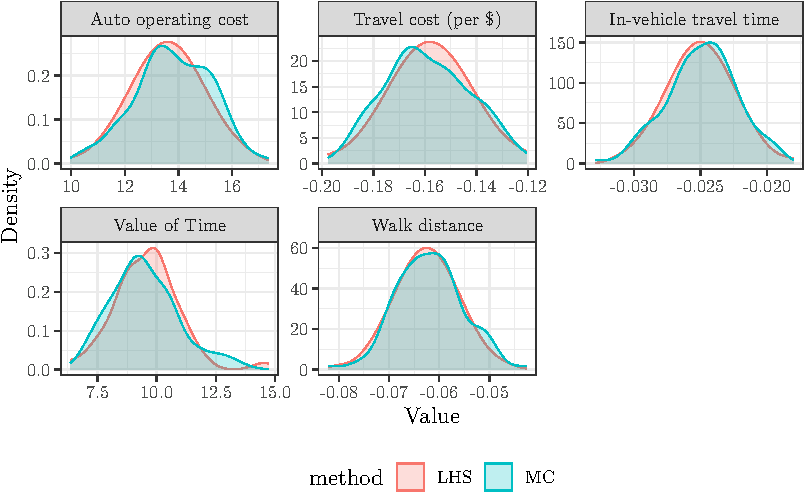
\includegraphics[keepaspectratio]{03-methods_files/figure-pdf/fig-parameter-1.pdf}}

}

\subcaption{\label{fig-parameter-1}100 draws}

\end{minipage}%
\newline
\begin{minipage}{\linewidth}

\centering{

\pandocbounded{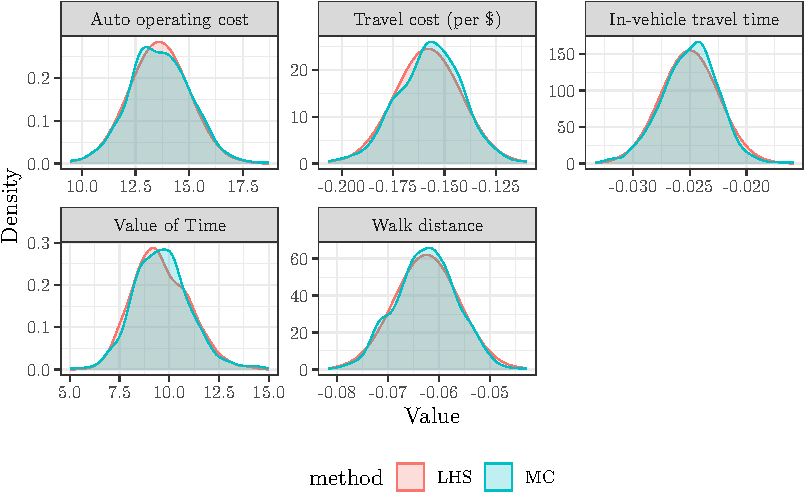
\includegraphics[keepaspectratio]{03-methods_files/figure-pdf/fig-parameter-2.pdf}}

}

\subcaption{\label{fig-parameter-2}600 draws}

\end{minipage}%

\caption{\label{fig-parameter}Sampled mode and destination choice
parameters for HBW trip purpose.}

\end{figure}%

To determine if LHS is effective at a reasonable amount of iterations,
the cumulative mean and the cumulative standard deviation of the average
MCLS value for every zone (see Equation~\ref{eq-mcls} ) was calculated
for each additional draw for both sampling methods. MCLS is an impedance
term which is an important value for destination choice and region
routing. The average MCLS, \(x\), was used as a measure of outcome
possibilities to simplify a complex term as a single value to compare by
across all iterations. The cumulative mean is calculated as:
\begin{equation}\phantomsection\label{eq-cmclsmean}{
\mu_i = \frac{x_1 + ... + x_i}{n}
}\end{equation} and the cumulative standard deviation is calculated as:
\begin{equation}\phantomsection\label{eq-sdi}{
SD_i = \sqrt{\frac{\sum (x_i - \mu_i)^2 }{n-1}}.
}\end{equation} The cumulative mean shows how the average MCLS
stabilizes across each iteration, and the cumulative standard deviation
is used to show the 95\% confidence interval of that mean. When the
cumulative mean for the draws stabilizes, that shows that the amount of
generated parameters has captured the possible variance of the results.
This is shown for two of the three trip purposes in Figure~\ref{fig-cm}.

\begin{sidewaysfigure}

\begin{minipage}{\linewidth}

\centering{

\pandocbounded{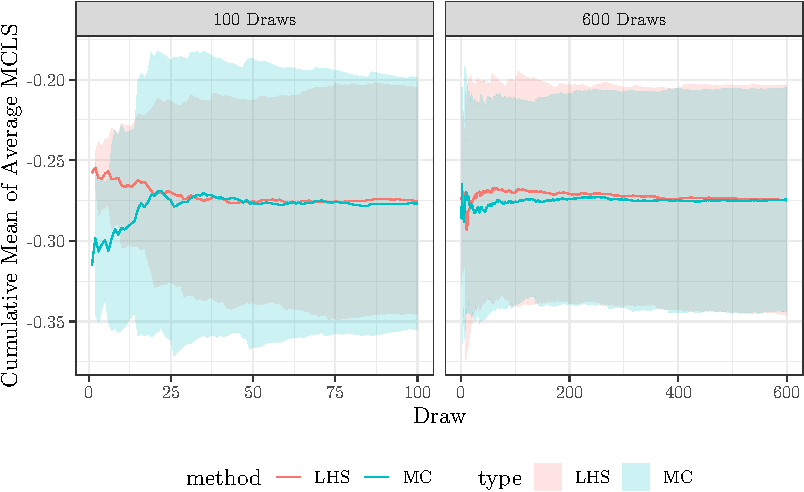
\includegraphics[keepaspectratio]{03-methods_files/figure-pdf/fig-cm-1.pdf}}

}

\subcaption{\label{fig-cm-1}HBW}

\end{minipage}%
\newline
\begin{minipage}{\linewidth}

\centering{

\pandocbounded{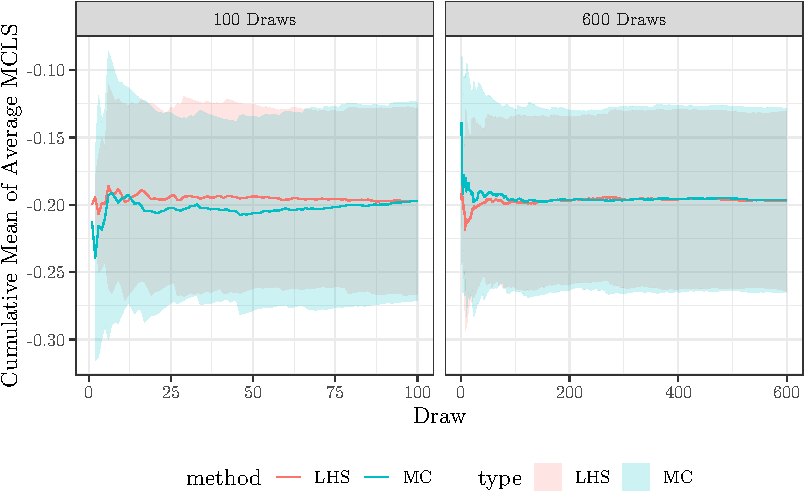
\includegraphics[keepaspectratio]{03-methods_files/figure-pdf/fig-cm-2.pdf}}

}

\subcaption{\label{fig-cm-2}HBO}

\end{minipage}%

\caption{\label{fig-cm}Average mode choice logsum (impedance) cumulative
mean and 95\% confidence interval with 100 and 600 draws.}

\end{sidewaysfigure}%

For all three trip purposes, both sampling methods had a stabilized mean
by 100 draws. The LHS methods standard deviation ribbon was generally
thinner than the MC method. From the narrowed cumulative standard
deviation, and that the parameter values are better normally distributed
when using LHS, that method of sampling was used for the assignment
analysis of the model. Since LHS captures the possible variance at a
small enough number of iterations, it can be used for large
transportation demand models. From these results it was decided to use
100 LHS samples parameters to evaluate uncertainty within each step of
the model. The next chapter includes the results of applying these
sampled parameters to the travel demand model.

\bookmarksetup{startatroot}

\section{Sensitivity Analysis Results}\label{sec-results}

Each of the 100 LHS parameter draws was applied to the RVTPO model,
generating mode choice utilities, destination choice utilities, and trip
matrices for each draw. The resulting uncertainty can then be quantified
using the outputs from the trip-based model. This section will first
look at the uncertainty of trips by mode, and how the mode split changes
when the parameters vary. Then uncertainty will be quantified using the
highway assigned trips, and how link volume changes across each draw.
The results will then be summarized.

\subsection{Mode Choice Trips}\label{mode-choice-trips}

Uncertainty can be evaluated by looking at how mode choices change. The
total number of trips by purpose are fixed, but the number of trips by
each mode changes as a result of mode choice, combined with the
availability of modes in the travel time skims. Table~\ref{tbl-mctrips}
lists the base trip amount by mode and purpose. It also lists the the
average number of trips across all 100 iterations, with the
corresponding standard deviation and coefficient of variation. For HBW
trips there are 103,320 auto trips. Across all 100 iterations there is a
mean value of 103,298 trips with a standard deviation of 527.07. This
results in a coefficient of variation of 0.0052 or 0.52\% variation in
the number of auto trips. The other modes of transportation are included
and similar patterns can be seen in HBO and NHB. The results listed in
the table show that the variation of the output trips - by mode and
purpose - are less than the input variation (as all \(c_v\)'s are
smaller than 0.10). This confirms previous research that the outcome
variance is less than or near the parameters variance (Clay and
Johnston, 2005; Zhao and Kockelman, 2002). In all three purposes that
were evaluated, the coefficient of variation in auto trips are lower
than transit or non-motorized trips, meaning that there is greater
confidence in the models accuracy to generate auto trips. The input
parameter variability has a smaller effect on auto trips than on trips
on the other modes.

\begin{longtable}[t]{lrrrr}

\caption{\label{tbl-mctrips}Coefficient of Variation of Trips by Mode}

\tabularnewline

\toprule
 & Base & Mean & SD & \$c\_v\$\\
\midrule
\addlinespace[0.3em]
\multicolumn{5}{l}{\textbf{HBW}}\\
\hspace{1em}Auto & 103320 & 103298 & 537.07 & 0.0052\\
\hspace{1em}Non-Motorized & 1103 & 1105 & 50.38 & 0.0456\\
\hspace{1em}Transit & 13254 & 13274 & 566.01 & 0.0426\\
\addlinespace[0.3em]
\multicolumn{5}{l}{\textbf{HBO}}\\
\hspace{1em}Auto & 250489 & 250475 & 453.11 & 0.0018\\
\hspace{1em}Non-Motorized & 4310 & 4316 & 235.24 & 0.0545\\
\hspace{1em}Transit & 9276 & 9283 & 363.09 & 0.0391\\
\addlinespace[0.3em]
\multicolumn{5}{l}{\textbf{NHB}}\\
\hspace{1em}Auto & 60212 & 60209 & 78.28 & 0.0013\\
\hspace{1em}Non-Motorized & 736 & 737 & 35.77 & 0.0485\\
\hspace{1em}Transit & 1576 & 1579 & 74.89 & 0.0474\\
\bottomrule

\end{longtable}

The variation among mode choices can be visualized graphically using a
density of a scaled change in trips by mode.
Figure~\ref{fig-modechoicetrips} shows density plots for HBW trips by
mode for 12 zones -- the zones are divided into three volume categories:
low is less than 200 trips per zone, mid is 200 to 700 trips per zone,
and top is greater than 700 trips per zone -- and four zones are
randomly selected from each volume category. Zones that do not have any
transit accessibility have been excluded. Those zones have very high
density in auto trips as with the ability to choose transit was removed,
the choice to choose auto was more certain. The zones included in
Figure~\ref{fig-modechoicetrips} all have greater certainty in auto
trips, as the change in trips across all 100 iterations is relatively
small. This reinforces the previous claim that the model has more
confidence in auto trips than the other modes. It is also important to
note that the modes are correlated to each other. In zones with a
greater confidence in one mode, the other modes are more confident as
well. Since the number of trips by origin zone are held constant, when
there are an increase in trips on one mode there must be a decrease in
trips on one or both of the other modes. Also, the distribution of
non-motorized trips is similar for every zone suggesting that generally,
the most variable mode is non-motorized trips which you can see in the
spread of the graphic. This is also verified using
Table~\ref{tbl-mctrips} as the \(c_v\) is largest for the non-motorized
mode across all three purposes.

\begin{sidewaysfigure}

\centering{

\pandocbounded{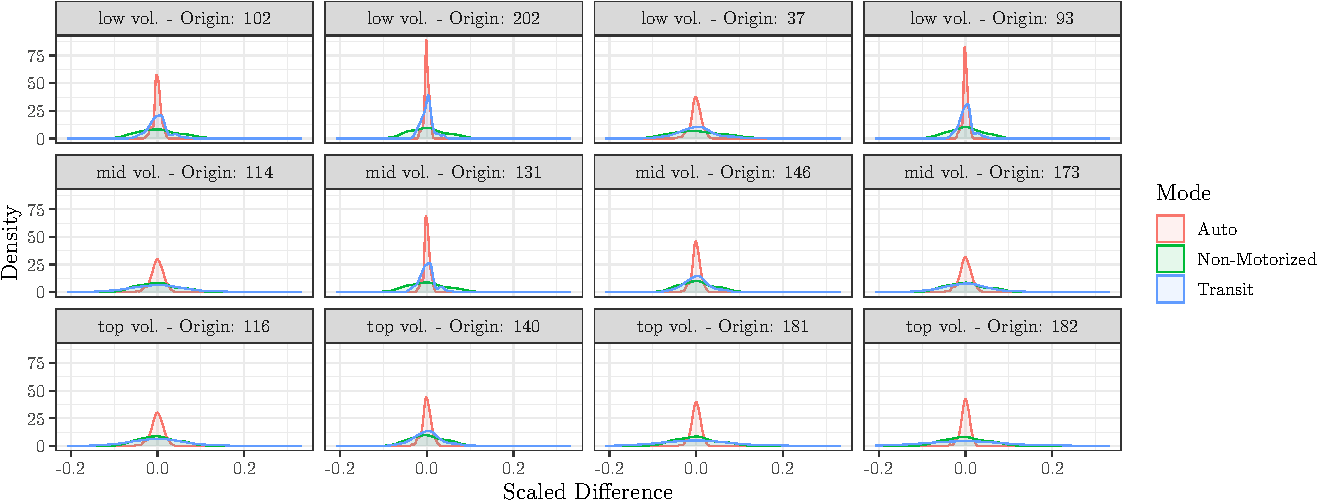
\includegraphics[keepaspectratio]{04-results_files/figure-pdf/fig-modechoicetrips-1.pdf}}

}

\caption{\label{fig-modechoicetrips}Trip density for coefficient of
variation by mode for HBW trips.}

\end{sidewaysfigure}%

\subsection{Link Volume}\label{link-volume}

Highway volumes are the most commonly used output of a travel model.
Uncertainty can additionally be evaluated by looking at how assigned
link volume varies across iterations. Figure~\ref{fig-networksd}
displays variation in forecast link volume spatially. This shows that
the links with the highest standard deviation in forecast volume are
high-volume roads including freeways and principal arterials where the
majority of traffic is internal to the study region. Although these
links have the largest standard deviation, when compared to the total
volume of the road, the variation is in reality very small. A standard
deviation of 400 vehicles on a road with 40,000 total vehicles
corresponds to a small variation (1\%).

\begin{sidewaysfigure}

\centering{

\pandocbounded{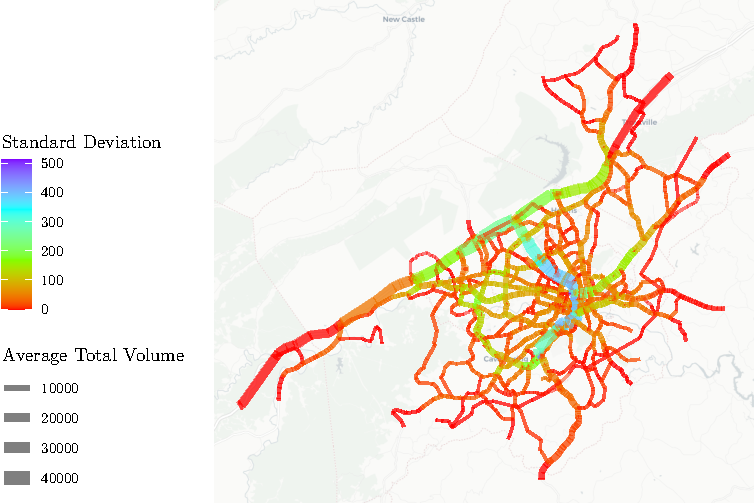
\includegraphics[keepaspectratio]{04-results_files/figure-pdf/fig-networksd-1.pdf}}

}

\caption{\label{fig-networksd}Standard deviation in daily forecast
volume.}

\end{sidewaysfigure}%

The highway assignment results can be grouped by facility type to show
how the coefficient of variation compares to link volume.
Figure~\ref{fig-totalvolume} shows the coefficient of variation for the
daily volume assigned to each network link, across the 100 draws,
plotted against the mean forecast link volume for each link. The values
are the volume for 100 randomly sampled links for each facility type.
The plots shows that for the high-volume roads such as major arterials
and freeways, the coefficient of variation converges to approximately
0.01, or about 1\% of the road's total forecast volume. For lower-volume
links, the coefficient of variation is more widely distributed, with
some local roads and small collectors having considerably higher values.
Some links in the model show no variation at all; these are presumably
links near the edges of the model region where the only traffic is to
and from external zones, trips which were held constant in this
framework.

\begin{figure}

\centering{

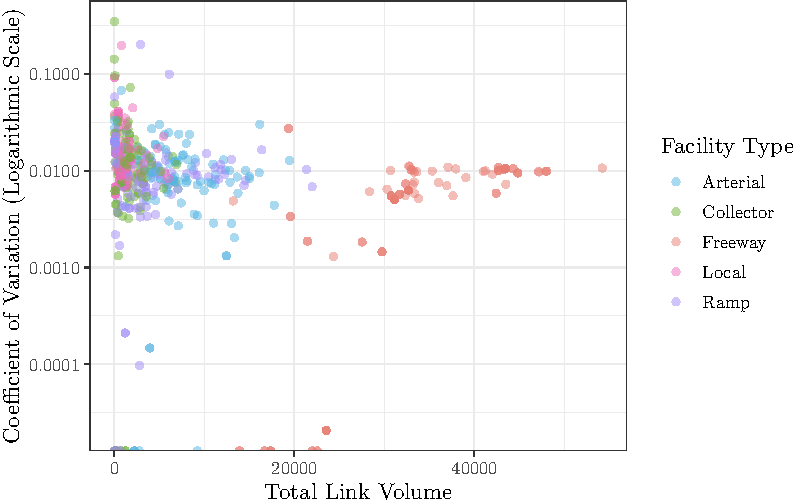
\includegraphics[width=1\linewidth,height=\textheight,keepaspectratio]{04-results_files/figure-pdf/fig-totalvolume-1.pdf}

}

\caption{\label{fig-totalvolume}Coefficient of variation in daily link
volume by facility type for a random sample of highway links.}

\end{figure}%

Variation among a link can also be visualized with a density plot of the
total volume across all iterations, as shown in
Figure~\ref{fig-densityplots}. In this plot, the density of forecast
volumes in three randomly selected links in each of the freeway,
collector, and arterial functional types are plotted alongside the
baseline forecast and the Average Annual Weekday Daily Traffic (AAWDT)
measured by the Virginia Department of Transportation, and to which the
model estimates were calibrated. In all cases, the error or uncertainty
in the forecast is considerably narrower than the error inherent in the
model construction, as evidenced by the fact that the AAWDT target value
is well outside the bell curve created by the statistically varied
simulation forecasts.

As expected from using the base parameter values as the mean of the LHS
parameter sampling, the base results are at or near the median of the
statistical density for each link's volume. But it is notable that the
estimated volumes are not perfectly, normally distributed as might be
naively expected. In this case, the combined effects of the mode and
destination choice parameter sampling appear to be constrained by the
geographic specificity of the RVTPO model network: even when the demand
for trips changes between zone pairs, the realities of the highway
capacity, volume-delay, and static user equilibrium procedures may be
limiting the possibilities for forecast highway volumes.

\begin{figure}

\centering{

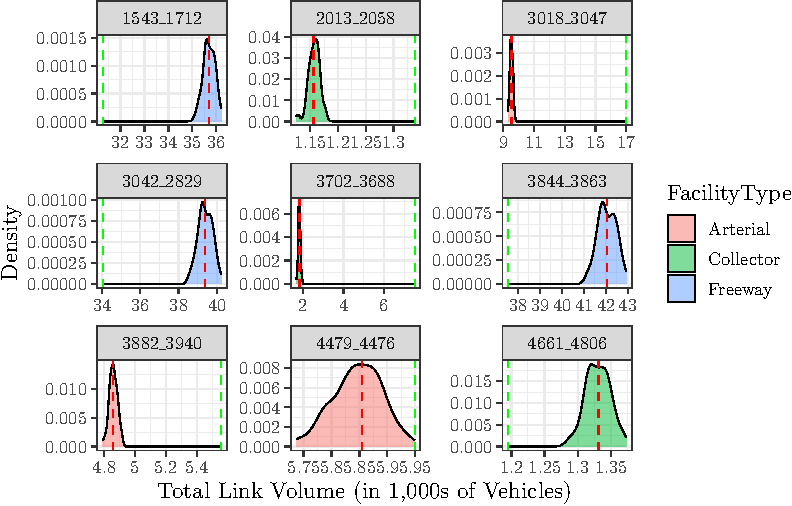
\includegraphics[width=1\linewidth,height=\textheight,keepaspectratio]{04-results_files/figure-pdf/fig-densityplots-1.pdf}

}

\caption{\label{fig-densityplots}Density plot of forecast volume on
selected links, with default parameter results marked in red, and AAWDT
values in green.}

\end{figure}%

\bookmarksetup{startatroot}

\section{Conclusions}\label{sec-conclusions}

In general, this research has shown that statistical parameter
uncertainty does not appear to be a significant factor in forecasting
traffic volumes using trip-based travel demand models. The result
uncertainty is generally equal to or smaller than the input parameter
variance. The uncertainty in parameter inputs appears to lead to
variation in highway volumes that is lower than the error between the
model forecast and the highway counts. Any variation in mode and
destination choice probabilities appears to be constrained by the
limitations of the highway network assignment.

There are several limitations that must be mentioned in this research,
however. First, we did not attempt to address the statistical
uncertainty in trip production estimates; these may play a substantially
larger role than destination and mode choice parameters, given that
lower trip rates may lead to lower traffic volumes globally, which could
not be ``corrected'' by the static user equilibrium assignment.
Additionally, the relatively sparse network of the RVTPO model region
--- lacking parallel high-capacity highway facilities --- may have meant
that the static network assignment would converge to a similar solution
point regardless of modest changes to the trip matrix. It may be that in
a larger network with more path redundancies, the assignment may not
have been as helpful in constraining the forecast volumes.

In this research we had only the estimates of the statistical
coefficients, and therefore had to assume a coefficient of variation to
derive variation in the sampling procedure. It would be better if model
user and development documentation more regularly provided estimates of
the standard errors of model parameters. Even better would be
variance-covariance matrices for the estimated models, enabling
researchers to ensure that covariance relationships between sampled
parameters are maintained.

Notwithstanding these limitations, statistical parameter variance does
not appear to be the largest source of uncertainty in travel
forecasting. There are likely more important factors at play that
planners and government agencies should address. Research on all sources
of uncertainty is somewhat limited, but in many ways has been hampered
by the burdensome computational requirements of many modern travel
models (Voulgaris, 2019). This research methodology benefited from a
lightweight travel model that could be repeatedly re-run with dozens of
sampled choice parameters. One strategy for applying this methodology to
larger models may be relatively recent TMIP-EMAT exploratory modeling
toolkit (Milkovits et al., 2019). But a better understanding the other
sources of uncertainty -- model specification and input accuracy --
might also benefit from lightweight models constructed for transparency
and flexibility rather than heavily constrained models emphasizing
precise spatial detail and strict behavioral constraints. This might
allow forecasts to be made with an ensemble approach (Wu and Levinson,
2021), identifying preferred policies as the consensus of multiple
plausible model specifications.

\bookmarksetup{startatroot}

\section*{Author Contribution
Statement}\label{author-contribution-statement}
\addcontentsline{toc}{section}{Author Contribution Statement}

\markboth{Author Contribution Statement}{Author Contribution Statement}

\textbf{Gregory S. Macfarlane:} Conceptualization, Methodology, Writing
- review \& editing, Supervision \textbf{Natalie M. Gray:} Methodology,
Software, Formal Analysis, Investigation, Writing - original draft,
Visualization

The authors have no competing interests in the publication of this
article, and the research received no external funding.

\bookmarksetup{startatroot}

\section*{References}\label{references}
\addcontentsline{toc}{section}{References}

\markboth{References}{References}

\phantomsection\label{refs}
\begin{CSLReferences}{1}{0}
\bibitem[\citeproctext]{ref-aep50_2023}
AEP50 Committee on Transportation Demand Forecasting, 2023. Uncertainty.

\bibitem[\citeproctext]{ref-armoogum2009}
Armoogum, J., Madre, J.-L., Bussiere, Y., 2009. Measuring uncertainty in
long-term travel demand forecasting from demographic modelling: {Case}
study of the {Paris} and {Montreal} metropolitan areas. IATSS research
33, 9--20.

\bibitem[\citeproctext]{ref-ben-akiva1985}
Ben-Akiva, M., Lerman, S.R., 1985.
\href{https://www.jstor.org/stable/1391567}{Discrete {Choice Analysis}:
{Theory} and {Applications} to {Travel Demand}}. MIT Press.

\bibitem[\citeproctext]{ref-clay2005univariate}
Clay, M.J., Johnston, R.A., 2005. Univariate uncertainty analysis of an
integrated land use and transportation model: {MEPLAN}. Transportation
Planning and Technology 28, 149--165.

\bibitem[\citeproctext]{ref-duthie2010highway}
Duthie, J., Voruganti, A., Kockelman, K., Waller, S.T., 2010. Highway
improvement project rankings due to uncertain model inputs:
{Application} of traditional transportation and land use models. Journal
of Urban Planning and Development 136, 294--302.

\bibitem[\citeproctext]{ref-flyvbjerg2005}
Flyvbjerg, B., Skamris Holm, M.K., Buhl, S.L., 2005. How ({In})accurate
{Are Demand Forecasts} in {Public Works Projects}?: {The Case} of
{Transportation}. Journal of the American Planning Association 71,
131--146. \url{https://doi.org/10.1080/01944360508976688}

\bibitem[\citeproctext]{ref-helton2003}
Helton, J.C., Davis, F.J., 2003. Latin hypercube sampling and the
propagation of uncertainty in analyses of complex systems. Reliability
Engineering \& System Safety 81, 23--69.
\url{https://doi.org/10.1016/S0951-8320(03)00058-9}

\bibitem[\citeproctext]{ref-hoque2021}
Hoque, J.M., Erhardt, G.D., Schmitt, D., Chen, M., Wachs, M., 2021.
Estimating the uncertainty of traffic forecasts from their historical
accuracy. Transportation Research Part A: Policy and Practice 147,
339--349. \url{https://doi.org/10.1016/j.tra.2021.03.015}

\bibitem[\citeproctext]{ref-koppelman2006}
Koppelman, F.S., Bhat, C., 2006. A {Self Instructing Course} in {Mode
Choice Modeling}: {Multinomial} and {Nested Logit Models}. Federal
Transit Administration.

\bibitem[\citeproctext]{ref-manzo2015}
Manzo, S., Nielsen, O.A., Prato, C.G., 2015. How uncertainty in input
and parameters influences transport model: Output {A} four-stage model
case-study. Transport Policy 38, 64--72.

\bibitem[\citeproctext]{ref-milkovits2019}
Milkovits, M., Copperman, R.B., Newman, J., Lemp, J., Rossi, T., United
States. Federal Highway Administration, 2019. {TMIP Exploratory
Modeling} and {Analysis Tool} ({TMIP-EMAT}) {Beta Test Results} (No.
FHWA-HEP-20-015).

\bibitem[\citeproctext]{ref-nationalacademiesofsciencesengineeringandmedicine.2012}
National Academies of Sciences, Engineering, and Medicine., 2012. Travel
{Demand Forecasting}: {Parameters} and {Techniques} (No. NCHRP 716).
National Academies Press, Washington, D.C.
\url{https://doi.org/10.17226/14665}

\bibitem[\citeproctext]{ref-petrik2020uncertainty}
Petrik, O., Adnan, M., Basak, K., Ben-Akiva, M., 2020. Uncertainty
analysis of an activity-based microsimulation model for {Singapore}.
Future Generation Computer Systems 110, 350--363.

\bibitem[\citeproctext]{ref-petrik2016measuring}
Petrik, O., Moura, F., Silva, J. de A. e, 2016. Measuring uncertainty in
discrete choice travel demand forecasting models. Transportation
Planning and Technology 39, 218--237.

\bibitem[\citeproctext]{ref-rasouli2012}
Rasouli, S., Timmermans, H., 2012. Uncertainty in travel demand
forecasting models: Literature review and research agenda.
Transportation Letters 4, 55--73.
\url{https://doi.org/10.3328/TL.2012.04.01.55-73}

\bibitem[\citeproctext]{ref-rodier2002uncertain}
Rodier, C.J., Johnston, R.A., 2002. Uncertain socioeconomic projections
used in travel demand and emissions models: Could plausible errors
result in air quality nonconformity? Transportation Research Part A:
Policy and Practice 36, 613--631.

\bibitem[\citeproctext]{ref-voulgaris2019}
Voulgaris, C.T., 2019. Crystal {Balls} and {Black Boxes}: {What Makes} a
{Good Forecast}? Journal of Planning Literature 34, 286--299.
\url{https://doi.org/10.1177/0885412219838495}

\bibitem[\citeproctext]{ref-welde2011planners}
Welde, M., Odeck, J., 2011. Do planners get it right? {The} accuracy of
travel demand forecasting in {Norway}. European Journal of Transport and
Infrastructure Research 11.

\bibitem[\citeproctext]{ref-wu2021}
Wu, H., Levinson, D., 2021. The ensemble approach to forecasting: {A}
review and synthesis. Transportation Research Part C: Emerging
Technologies 132, 103357.
\url{https://doi.org/10.1016/j.trc.2021.103357}

\bibitem[\citeproctext]{ref-yang2013}
Yang, C., Chen, A., Xu, X., Wong, S.C., 2013. Sensitivity-based
uncertainty analysis of a combined travel demand model. Transportation
Research Part B: Methodological 57, 225--244.
\url{https://doi.org/10.1016/j.trb.2013.07.006}

\bibitem[\citeproctext]{ref-zhao2002}
Zhao, Y., Kockelman, K.M., 2002. The propagation of uncertainty through
travel demand models: {An} exploratory analysis. The Annals of Regional
Science 36, 145--163. \url{https://doi.org/10.1007/s001680200072}

\end{CSLReferences}

%%%%%%%%%%%%%%%%%%%%%%%%%%%%%%%%%%%%%%%%%%









\PublishersNote{}
\end{document}
